\chapter{Introduction to Machine Learning}
\label{ch:ml_intro}

\section{What is Machine Learning?}

\begin{definition}[Machine Learning]
\textbf{Machine learning}\index{machine learning} (ML) is a branch of artificial intelligence that enables computers to learn from data without being explicitly programmed for each task.
\end{definition}

\begin{intuition}
Rather than writing rules manually (for example, ``if the customer is over 30 years old and has an income above \$50,000, then approve the loan''), we provide \textbf{examples} to the model, which discovers the underlying rules on its own.
\end{intuition}

\subsection{Types of Learning}

\index{supervised learning}\index{unsupervised learning}\index{reinforcement learning}

\begin{center}
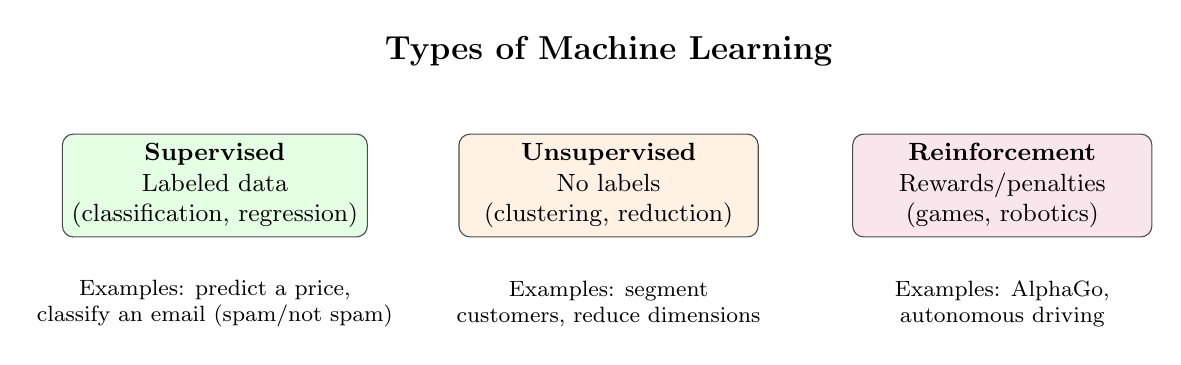
\begin{tikzpicture}[
    box/.style={rectangle, draw=black!70, fill=blue!8, rounded corners, minimum width=3.8cm, minimum height=1.2cm, align=center, font=\small},
    title/.style={font=\bfseries\large}
]
\node[title] at (0, 3.2) {Types of Machine Learning};
\node[align=center,box, fill=green!10] (sup) at (-5, 1.5) {\textbf{Supervised}\\Labeled data\\(classification, regression)};
\node[align=center,box, fill=orange!10] (unsup) at (0, 1.5) {\textbf{Unsupervised}\\No labels\\(clustering, reduction)};
\node[align=center,box, fill=purple!10] (reinf) at (5, 1.5) {\textbf{Reinforcement}\\Rewards/penalties\\(games, robotics)};

\node[font=\footnotesize, align=center] at (-5, 0) {Examples: predict a price,\\classify an email (spam/not spam)};
\node[font=\footnotesize, align=center] at (0, 0) {Examples: segment\\customers, reduce dimensions};
\node[font=\footnotesize, align=center] at (5, 0) {Examples: AlphaGo,\\autonomous driving};
\end{tikzpicture}
\end{center}

\begin{definition}[Supervised Learning]
We have pairs $(\mathbf{x}_i, y_i)$ where $\mathbf{x}_i$ are the \textbf{explanatory variables}\index{explanatory variables} (\textit{features}) and $y_i$ is the \textbf{target}\index{target}. The model learns a function $f$ such that $f(\mathbf{x}_i) \approx y_i$.
\begin{itemize}
    \item \textbf{Classification}\index{classification}: $y$ is a category (spam/not spam, flower species).
    \item \textbf{Regression}\index{regression}: $y$ is a continuous value (price, temperature).
\end{itemize}
\end{definition}

\begin{definition}[Unsupervised Learning]
We only have $\mathbf{x}_i$ without labels. The model seeks \textbf{hidden structures} in the data (groups, principal axes).
\end{definition}

\section{The Supervised Learning Workflow}
\label{sec:workflow_ml}

\index{train/test split}

\begin{center}
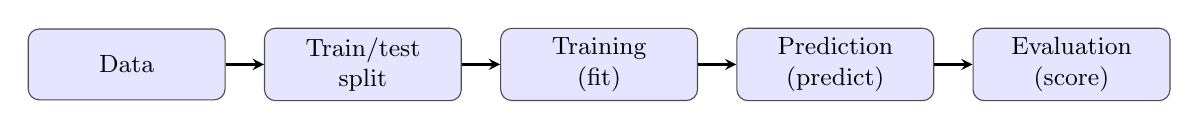
\begin{tikzpicture}[
    stepbox/.style={rectangle, draw=black!70, fill=blue!10, rounded corners, minimum width=2.5cm, minimum height=0.9cm, align=center, font=\small},
    arr/.style={->, thick, >=stealth}
]
\node[stepbox] (data) at (0,0) {Data};
\node[align=center,stepbox] (split) at (3,0) {Train/test\\split};
\node[align=center,stepbox] (train) at (6,0) {Training\\(\py{fit})};
\node[align=center,stepbox] (pred) at (9,0) {Prediction\\(\py{predict})};
\node[align=center,stepbox] (eval) at (12,0) {Evaluation\\(\py{score})};

\draw[arr] (data) -- (split);
\draw[arr] (split) -- (train);
\draw[arr] (train) -- (pred);
\draw[arr] (pred) -- (eval);
\end{tikzpicture}
\end{center}

\begin{enumerate}
    \item \textbf{Collect and prepare} the data.
    \item \textbf{Split} into a training set\index{training set} and a test set\index{test set}.
    \item \textbf{Train} the model on the training data.
    \item \textbf{Predict} on the test data.
    \item \textbf{Evaluate} the performance.
\end{enumerate}

\begin{codeblock}[title=\textbf{Python}]
\begin{minted}{python}
from sklearn.model_selection import train_test_split
from sklearn.datasets import load_iris

# Load the data
iris = load_iris()
X, y = iris.data, iris.target

# Split: 70% training, 30% test
X_train, X_test, y_train, y_test = train_test_split(
    X, y, test_size=0.3, random_state=42
)
print(f"Training: {X_train.shape[0]} samples")
print(f"Test: {X_test.shape[0]} samples")
\end{minted}
\end{codeblock}

\begin{codeoutput}
\begin{minted}{text}
Training: 105 samples
Test: 45 samples
\end{minted}
\end{codeoutput}

\section{The Scikit-learn API}
\label{sec:api_sklearn}

\index{scikit-learn}\index{fit}\index{predict}\index{score}

\begin{bestpractice}
All scikit-learn models follow the same interface:
\begin{enumerate}
    \item \py{model = Class(parameters)} --- create the model.
    \item \py{model.fit(X_train, y_train)} --- train.
    \item \py{model.predict(X_test)} --- predict.
    \item \py{model.score(X_test, y_test)} --- evaluate.
\end{enumerate}
\end{bestpractice}

\subsection{Complete Example: k-Nearest Neighbors on Iris}

\index{k-nearest neighbors}\index{KNN}

\begin{codeblock}[title=\textbf{Python}]
\begin{minted}{python}
from sklearn.neighbors import KNeighborsClassifier
from sklearn.metrics import accuracy_score

# Create the KNN model with k=5
knn = KNeighborsClassifier(n_neighbors=5)

# Training
knn.fit(X_train, y_train)

# Prediction
y_pred = knn.predict(X_test)

# Evaluation
acc = accuracy_score(y_test, y_pred)
print(f"Predictions: {y_pred[:10]}")
print(f"True values: {y_test[:10]}")
print(f"Accuracy:    {acc:.4f}")
\end{minted}
\end{codeblock}

\begin{codeoutput}
\begin{minted}{text}
Predictions: [1 0 2 1 1 0 1 2 1 1]
True values: [1 0 2 1 1 0 1 2 1 1]
Accuracy:    1.0000
\end{minted}
\end{codeoutput}

\begin{remark}
The \py{score()} method returns the \textbf{accuracy}\index{accuracy} for classification and the \textbf{coefficient of determination} $R^2$ for regression.
\end{remark}

\section{Overfitting and Underfitting}
\label{sec:overfitting}

\index{overfitting}\index{underfitting}\index{bias}\index{variance}

\begin{definition}[Overfitting and Underfitting]
\begin{itemize}
    \item \textbf{Underfitting}\index{underfitting}: the model is too simple and fails to capture the structure of the data. \textbf{High bias}.
    \item \textbf{Overfitting}\index{overfitting}: the model is too complex and memorizes the noise in the training data. \textbf{High variance}.
\end{itemize}
\end{definition}

\begin{center}
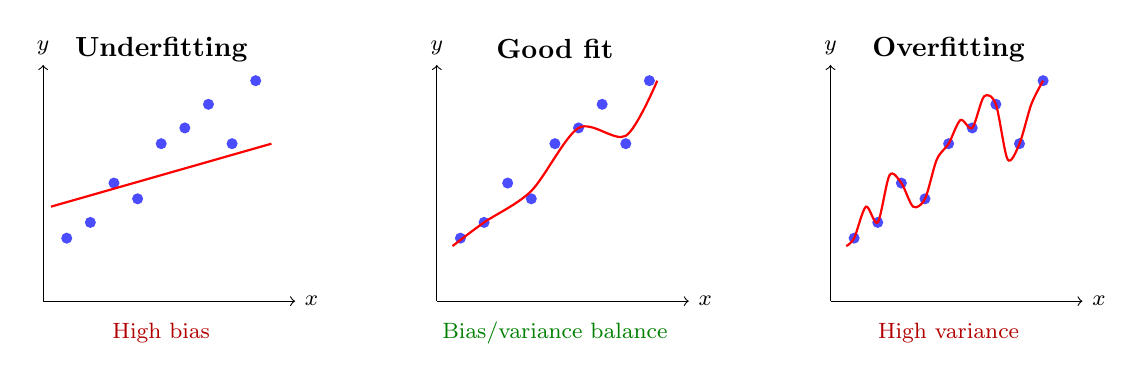
\begin{tikzpicture}
    % Underfitting
    \begin{scope}[shift={(-5,0)}]
        \node[font=\bfseries] at (1.5, 3.2) {Underfitting};
        \draw[->] (0,0) -- (3.2,0) node[right] {\footnotesize $x$};
        \draw[->] (0,0) -- (0,3) node[above] {\footnotesize $y$};
        \foreach \x/\y in {0.3/0.8, 0.6/1.0, 0.9/1.5, 1.2/1.3, 1.5/2.0, 1.8/2.2, 2.1/2.5, 2.4/2.0, 2.7/2.8} {
            \fill[blue!70] (\x, \y) circle (2pt);
        }
        \draw[red, thick] (0.1, 1.2) -- (2.9, 2.0);
        \node[font=\footnotesize, text=red!70!black] at (1.5, -0.4) {High bias};
    \end{scope}
    % Good fit
    \begin{scope}[shift={(0,0)}]
        \node[font=\bfseries] at (1.5, 3.2) {Good fit};
        \draw[->] (0,0) -- (3.2,0) node[right] {\footnotesize $x$};
        \draw[->] (0,0) -- (0,3) node[above] {\footnotesize $y$};
        \foreach \x/\y in {0.3/0.8, 0.6/1.0, 0.9/1.5, 1.2/1.3, 1.5/2.0, 1.8/2.2, 2.1/2.5, 2.4/2.0, 2.7/2.8} {
            \fill[blue!70] (\x, \y) circle (2pt);
        }
        \draw[red, thick, smooth] plot coordinates {(0.2, 0.7) (0.6, 1.0) (1.2, 1.4) (1.8, 2.2) (2.4, 2.1) (2.8, 2.8)};
        \node[font=\footnotesize, text=green!50!black] at (1.5, -0.4) {Bias/variance balance};
    \end{scope}
    % Overfitting
    \begin{scope}[shift={(5,0)}]
        \node[font=\bfseries] at (1.5, 3.2) {Overfitting};
        \draw[->] (0,0) -- (3.2,0) node[right] {\footnotesize $x$};
        \draw[->] (0,0) -- (0,3) node[above] {\footnotesize $y$};
        \foreach \x/\y in {0.3/0.8, 0.6/1.0, 0.9/1.5, 1.2/1.3, 1.5/2.0, 1.8/2.2, 2.1/2.5, 2.4/2.0, 2.7/2.8} {
            \fill[blue!70] (\x, \y) circle (2pt);
        }
        \draw[red, thick, smooth] plot coordinates {(0.2, 0.7) (0.3, 0.8) (0.45, 1.2) (0.6, 1.0) (0.75, 1.6) (0.9, 1.5) (1.05, 1.2) (1.2, 1.3) (1.35, 1.8) (1.5, 2.0) (1.65, 2.3) (1.8, 2.2) (1.95, 2.6) (2.1, 2.5) (2.25, 1.8) (2.4, 2.0) (2.55, 2.5) (2.7, 2.8)};
        \node[font=\footnotesize, text=red!70!black] at (1.5, -0.4) {High variance};
    \end{scope}
\end{tikzpicture}
\end{center}

\begin{theorem}[Bias-Variance Tradeoff]
The generalization error\index{generalization error} of a model decomposes into:
\[
\text{Total error} = \text{Bias}^2 + \text{Variance} + \text{Irreducible noise}
\]
The goal is to find the model that minimizes this total error by balancing bias and variance.
\end{theorem}

\begin{center}
\begin{tikzpicture}
    \draw[->] (0,0) -- (8,0) node[right] {Model complexity};
    \draw[->] (0,0) -- (0,5) node[above] {Error};
    \draw[blue, thick, domain=0.5:7.5, smooth] plot (\x, {3.5/\x + 0.3});
    \node[blue, font=\footnotesize] at (2.5, 2.5) {Bias$^2$};
    \draw[red, thick, domain=0.5:7.5, smooth] plot (\x, {0.05*\x*\x + 0.2});
    \node[red, font=\footnotesize] at (6, 2.5) {Variance};
    \draw[black!60, thick, dashed, domain=0.5:7.5, smooth] plot (\x, {3.5/\x + 0.05*\x*\x + 0.5});
    \node[black!60, font=\footnotesize] at (5.5, 4.5) {Total error};
    \draw[green!50!black, thick, dashed] (2.8, 0) -- (2.8, 4.5);
    \node[green!50!black, font=\footnotesize, align=center] at (2.8, 4.8) {Optimum};
\end{tikzpicture}
\end{center}

\section{Cross-Validation}
\label{sec:cross_validation}

\index{cross-validation}\index{k-fold}

\begin{definition}[$k$-Fold Cross-Validation]
\textbf{Cross-validation} ($k$-fold cross-validation) divides the data into $k$ subsets (\textit{folds}). The model is trained $k$ times, each time using a different fold as the test set and the remaining $k-1$ folds as the training set.
\end{definition}

\begin{center}
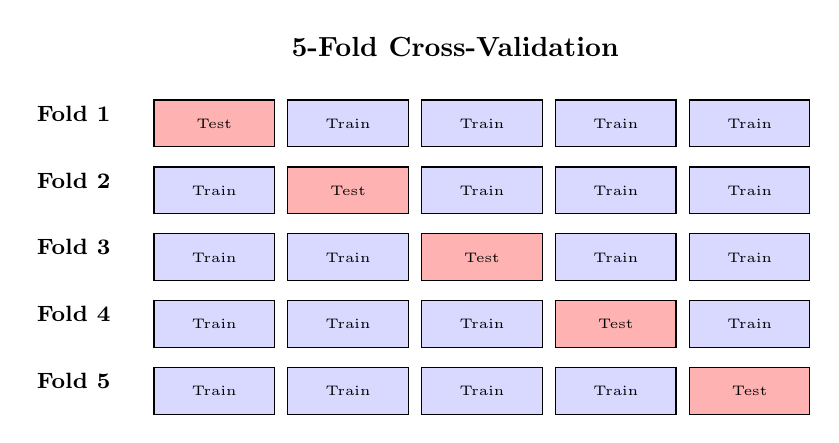
\begin{tikzpicture}[scale=0.85]
    \foreach \fold in {1,...,5} {
        \pgfmathtruncatemacro{\ypos}{-\fold}
        \node[font=\footnotesize\bfseries] at (-1.2, \ypos+0.5) {Fold \fold};
        \foreach \block in {1,...,5} {
            \pgfmathtruncatemacro{\xpos}{(\block-1)*2}
            \ifnum\block=\fold
                \fill[red!30] (\xpos, \ypos) rectangle (\xpos+1.8, \ypos+0.7);
                \draw (\xpos, \ypos) rectangle (\xpos+1.8, \ypos+0.7);
                \node[font=\tiny] at (\xpos+0.9, \ypos+0.35) {Test};
            \else
                \fill[blue!15] (\xpos, \ypos) rectangle (\xpos+1.8, \ypos+0.7);
                \draw (\xpos, \ypos) rectangle (\xpos+1.8, \ypos+0.7);
                \node[font=\tiny] at (\xpos+0.9, \ypos+0.35) {Train};
            \fi
        }
    }
    \node[font=\bfseries] at (4.5, 0.5) {5-Fold Cross-Validation};
\end{tikzpicture}
\end{center}

\begin{codeblock}[title=\textbf{Python}]
\begin{minted}{python}
from sklearn.model_selection import cross_val_score

knn = KNeighborsClassifier(n_neighbors=5)

# 5-fold cross-validation
scores = cross_val_score(knn, X, y, cv=5, scoring='accuracy')

print(f"Scores per fold: {scores}")
print(f"Mean: {scores.mean():.4f}")
print(f"Std: {scores.std():.4f}")
\end{minted}
\end{codeblock}

\begin{codeoutput}
\begin{minted}{text}
Scores per fold: [0.9667 0.9667 0.9333 0.9667 1.0000]
Mean: 0.9667
Std: 0.0211
\end{minted}
\end{codeoutput}

\begin{warning}
Never evaluate a model on the training data! A perfect score on the training set may hide severe \textbf{overfitting}. Always use a separate test set or cross-validation.
\end{warning}

\subsection{Choosing $k$ in KNN}

\begin{codeblock}[title=\textbf{Python}]
\begin{minted}{python}
import numpy as np

k_values = range(1, 21)
mean_scores = []

for k in k_values:
    knn = KNeighborsClassifier(n_neighbors=k)
    scores = cross_val_score(knn, X, y, cv=5)
    mean_scores.append(scores.mean())

best_k = k_values[np.argmax(mean_scores)]
print(f"Best k: {best_k}")
print(f"Best score: {max(mean_scores):.4f}")
\end{minted}
\end{codeblock}

\begin{codeoutput}
\begin{minted}{text}
Best k: 6
Best score: 0.9800
\end{minted}
\end{codeoutput}

\section{Exercises}

\begin{exercise}[$\star$]
Load the \py{load_wine()} dataset from scikit-learn. Split it into 80\%/20\%, train a KNN with $k=3$, and display the accuracy on the test set.
\end{exercise}

\begin{exercise}[$\star$]
Explain in your own words the difference between overfitting and underfitting. Give a concrete example for each.
\end{exercise}

\begin{exercise}[$\star\star$]
On the Iris dataset, compare the performance of KNN for $k \in \{1, 3, 5, 7, 9, 11\}$ using 10-fold cross-validation. Plot a graph of mean scores as a function of $k$.
\end{exercise}

\begin{exercise}[$\star\star$]
Load the \py{load_digits()} dataset and perform classification with KNN. Compute the 5-fold cross-validation. What do you notice about the performance?
\end{exercise}

\begin{exercise}[$\star\star\star$]
Load the \texttt{penguins} dataset from seaborn. Prepare the data (remove missing values, encode categorical variables with \py{pd.get_dummies}). Train a KNN to predict the species and evaluate with cross-validation. Compare the performance with and without data normalization (\py{StandardScaler}).
\end{exercise}

\begin{exercise}[$\star\star\star$]
Create a synthetic dataset with \py{make_classification(n_samples=500, n_features=20, n_informative=5)}. Compare the training and test accuracy for a KNN with $k=1$ and $k=10$. Which one overfits more? Justify your answer.
\end{exercise}

\begin{keyformulas}
\textbf{Summary of Chapter~\ref{ch:ml_intro}}
\begin{itemize}
    \item \textbf{Supervised learning}: labeled data $(\mathbf{x}_i, y_i)$, classification or regression.
    \item \textbf{Unsupervised learning}: no labels, structure discovery.
    \item \textbf{Scikit-learn API}: \py{fit(X_train, y_train)}, \py{predict(X_test)}, \py{score(X_test, y_test)}.
    \item \textbf{Splitting}: \py{train_test_split(X, y, test_size=0.3, random_state=42)}.
    \item \textbf{Overfitting}: model too complex, high variance.
    \item \textbf{Underfitting}: model too simple, high bias.
    \item \textbf{Bias-variance tradeoff}: $\text{Error} = \text{Bias}^2 + \text{Variance} + \text{Noise}$.
    \item \textbf{Cross-validation}: \py{cross_val_score(model, X, y, cv=k)}, robust estimation.
\end{itemize}
\end{keyformulas}
